\section{Simulator Implementation}
We implemented two versions of a simulator of our system: 
\begin{enumerate}
\item An offline simulator, which uses data collected and stored during a mobile browsing session, and input into the simulator offline, and
\item A networked simulator, which simulates a basic incarnation of our system in real-time.
\end{enumerate}
Both simulators are written in Java, and use five helper interfaces and classes each one representing a component of the system, in addition to the proxy server and mobile device classes. In particular, we use two helper interfaces: \texttt{ICache} and \texttt{IProcessor}, which allow for different implementations of caches supporting various eviction algorithms, and of what we call cache processors, respectively. A cache processor is an entity which acts as an interface between a device and its web cache, with its most important task to process incoming web content based on the device's cache contents. While both of our simulators use a simple implementation of \texttt{IProcessor} called \texttt{SimpleProcessor}, which manages web content caching, and measures the cache hitrate and missrate, we have multiple implementations of \texttt{ICache}, which we address later in this section. 

The three helper functions we use are \texttt{Chunk}, \texttt{Chunking} and \texttt{Fingerprinting}. The \texttt{Chunk} class defines a fixed-size data chunk with a given size in number of bytes and the data. \texttt{Chunking} is the facility which generates all the data chunks for a given input, either an input file containing web page data or a data stream of online web data. The \texttt{Fingerprinting} class is a wrapper for the Java \emph{rabinhash} library written by Sean Owen \cite{rabinhash}, and uses the \texttt{RabinHashFunction32} implementation of Rabin's fingerprinting method creating 32-bit fingerprints of a given data chunk \cite{rabin_api}.

Finally, we created the \texttt{ISimulator} interface to build different kinds of simulators. Our offline version uses one or more \texttt{Mobile} devices and a \texttt{ProxyServer} to implement the simulation of our reduction protocol described in Section \ref{sec:protocol}. The networked simulator uses the networked counterparts of these two components.
\subsection{Offline Simulator}
\subsection{Networked Simulator}
\label{sec:netsim}
The networked simulator consists of the proxy server (\texttt{ProxyServerNet}) and the mobile client simulator (\texttt{SimulatorV3} run on a departmental Ubuntu server), which is a wrapper for the networked mobile proxy-client (\texttt{MobileClientNet}) and is capable of performing several rounds of requests to the proxy server in real-time. It does so by prompting the user to manually enter the next web page URL she wishes to visit, simulating web browser interactions (see Figure \ref{fig:mobsim_ui} for an example of the user interface of our mobile client). The simulator architecture can be seen in Figure \ref{fig:netsim_arch}. 

\begin{figure*}[ht] 
\centering 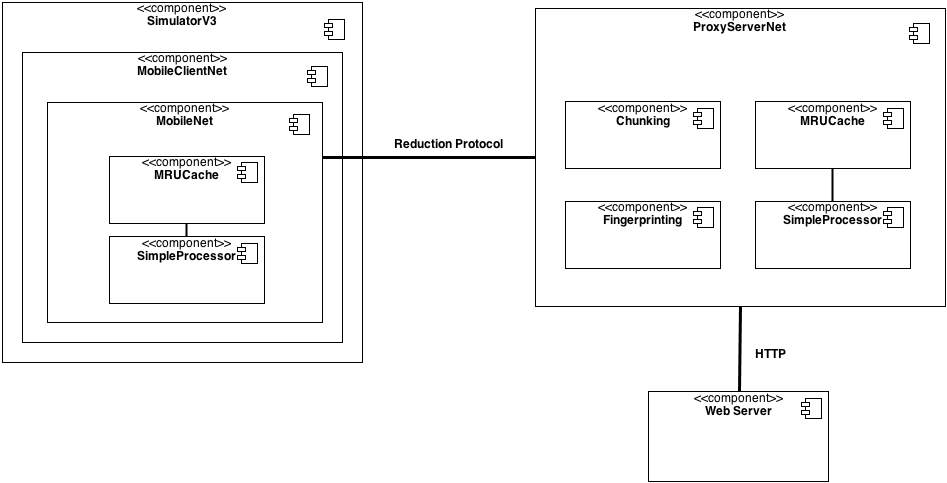
\includegraphics[scale=0.40]{images/component_diagram.png}
\caption{Networked Simulator Runtime Interactions.}
\label{fig:netsim_arch}
\end{figure*}

\begin{figure}[h] 
\centering 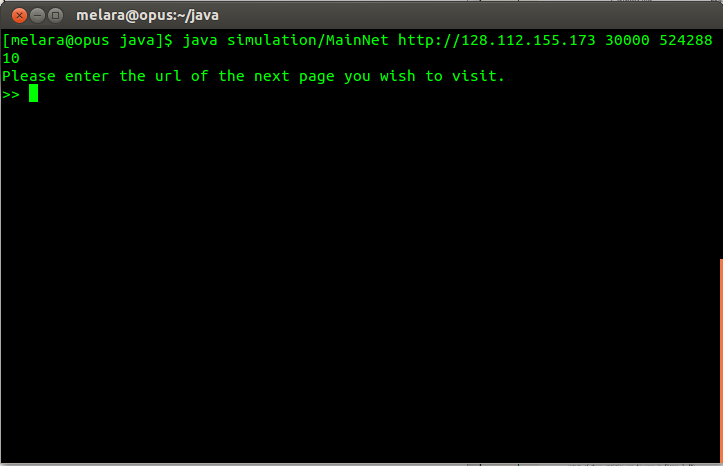
\includegraphics[scale=0.40]{images/mobilesim_ui.png}
\caption{The User Interface of our Mobile Client Simulator.}
\label{fig:mobsim_ui}
\end{figure}

In more detail, the networked simulator implements our reduction protocol as follows. First, the mobile proxy-client opens a socket to the proxy server, which is listening for connections at a user-specified port. The mobile proxy-client sends a simplified HTTP request of the format \emph{GET $<$url$>$ HTTP/1.1} to the proxy server. It then formulates a proper HTTP request, including the User-Agent string of a mobile device\footnote{We use the Samsung Galaxy SII as our model mobile device across all our implementations and experiments.} to ensure that it receives the mobile version of the requested web page from the hosting web server. Once the proxy has received the content of the requested page from the appropriate web server, it engages in the bandwidth reduction protocol\footnote{Minor changes were made to the chunking facility as well as the mobile device definition to support networking.} with the mobile proxy-client, exchanging the relevant information via the network. At the end, the mobile proxy-client reconstructs the content data of the received web page into an HTML file, which can then be viewed in any web browser. After the proxy has served the mobile client's request, the client is able to make a new request and repeat this process.

We found that, while simulating mobile browsing, for one not using an actual mobile phone, and for another not using a web browser program of any sort, is not realistic, our networked simulator is a good first proof-of-concept prototype showing that our reduction protocol is viable. In our experimental evaluation, we argue that it reduces the required bandwidth compared to the currently required mobile browsing bandwidth.

In the end, we would like to discuss some caveats of our networked simulator. First, as our mobile client simulator does not have the capabilities of a web browser and it receives preprocessed data from the proxy server, it cannot automatically handle HTTP responses indicating page redirects (i.e. server response code $301$, for example). Thus, our proxy server handles HTTP responses with the server response codes $200$ and $40X$\footnote{$200$ means granted normally, $40X$ response codes indicate a form of client-side error such as malformed requests but return HTML-format content with this information.} since the web server returns HTML content with these responses. An additional consequence of the fact that our mobile client is not browser-like is that it must create a local copy of each retrieved web page. Although the content of the web page is reconstructed correctly, since many links within web pages point to relative paths, the retrieved web pages are often rendered incorrectly in the local web browser as it cannot find cascading stylesheets (CSS) and embedded images on the local disk. We propose how to solve these issues in our discussion on future work.

\subsection{Using Different Caching Algorithms}
